%%=========================================
\thispagestyle{empty}
\includegraphics[scale=0.5]{Figures/ntnu_bredde_eng_svart.png}
\begin{center}
\vspace{2pc}
\Huge{TBA4251 Programmering i Geomatikk \\ Vektorbasert Klient-Server WebGIS }
\vspace{4pc}

    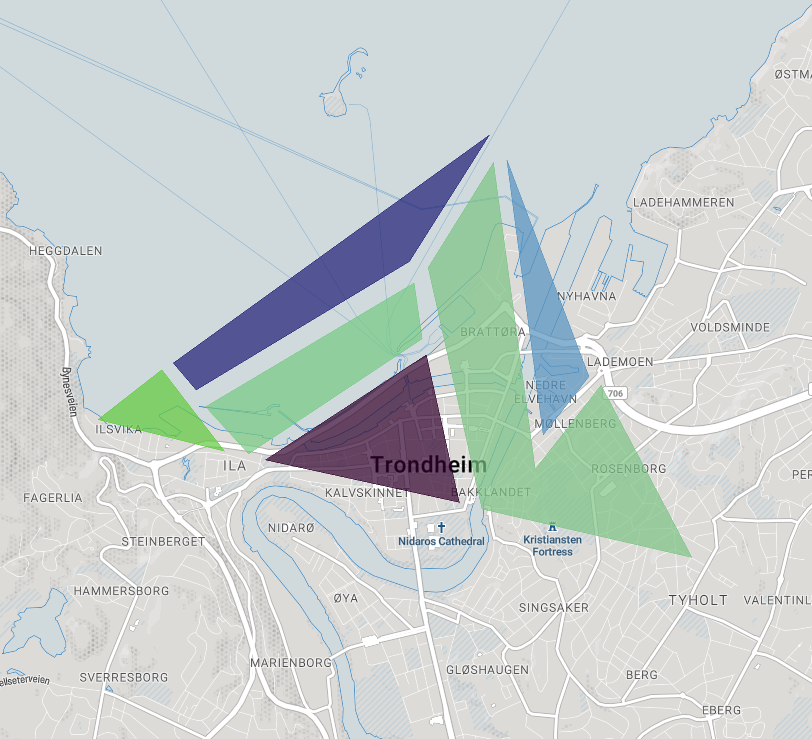
\includegraphics[scale=0.5]{Figures/forside.png}

\vspace{4pc}
\end{center}

Torstein Solberg\\
Programmering i Geomatikk\\
Institutt for bygg- og miljøteknikk\\
Norges Teknisk-Naturvitenskapelige Universitet

%\begin{info}
%	\textbf{Draft mode is ON}

%	Yellow boxes with info and tips for writing will appear.

%	Setting the draft option will speed up compilation of the PDF, because figures are not loaded, just indicated by a frame. Other package specific simplifications are also enabled, like removing hyperrefs. 

%	LaTeX will also inform you about hyphenation (Overfull hbox warning) and justification problems with a small black square. You can find these in the console after compiling.

%	\emph{To disable:} Delete the draft option or replace it with final in the final document version. This is done at the top of the \emph{main.tex} file.
%\end{info}

%%=========================================
